\documentclass[11pt]{article}
\usepackage[margin=1in]{geometry}
\usepackage{graphicx}
\usepackage{amsmath}
\usepackage{amssymb}
\usepackage{booktabs}
\usepackage{siunitx}
\usepackage{xcolor}
\usepackage{caption}
\usepackage[colorlinks=true,linkcolor=blue!55!black,urlcolor=blue!55!black]{hyperref}
\captionsetup{font=small,labelfont=bf}
\graphicspath{{figs/}}
\newcommand{\qx}{q_X}
\newcommand{\qy}{q_Y}
\newcommand{\fbal}{f}
\newcommand{\adc}{\,\mathrm{ADC}}

\title{\vspace{-1.5em}Charge balance between the X and Y readout layers of the
MX17 resistive Micromegas\\
\large June 2026 cosmic bench --- det3 (\texttt{sat\_det3}) with det2 cross-check}
\author{MX17 cosmic-bench analysis (paper topic 4)}
\date{2026-07-12}

\begin{document}
\maketitle
\vspace{-1.5em}

\begin{quote}\small\itshape
2026-07-14 note: the M3 reference recipe changed to $\chi^2<1.0$, $N_\mathrm{clus}=4$
(was $\chi^2<5$, $N_\mathrm{clus}\ge3$; see \texttt{M3\_CUT\_AND\_ACTIVE\_AREA\_NOTE.md}).
Script~38 was re-run for det3/det2 on the new recipe and the figures above are
regenerated from it; the quoted $\fbal$ medians/$\sigma_{68}$ in the text below shifted
by $<1\%$ (e.g.\ det3 median $0.487\to0.491$, $\sigma_{68}$ $0.067\to0.065$) --- within
rounding, conclusions unchanged, exact text digits not individually re-verified.
\end{quote}

\begin{abstract}
\noindent The MX17 chamber reads out two orthogonal strip layers (X on top, Y
beneath) that share a single avalanche through a pixelated resistive top layer.
We ask whether that top layer divides the charge \emph{evenly} and
\emph{stably} between the two layers --- the quantitative test that the readout
is well coupled. Defining the balance fraction $\fbal=\qx/(\qx+\qy)$ from the
per-plane charge sums, we find on the frozen June cosmic data that $\fbal$ is
narrow ($\sigma_{68}\approx0.07$), essentially independent of hit position
($<2\%$ real variation across the active area) and of track angle, with a
central value of $\fbal=0.487$ (det3) and $0.531$ (det2). The two chambers
differ by only ${\sim}0.04$ --- a small per-assembly offset, not a spread ---
and the charge is strongly correlated between layers ($r=0.88/0.85$). The result
is reproduced by three \emph{independent} charge estimators (saturation-corrected
peak amplitude, pulse integral, and the clustered unshared strip sum), whose
medians agree to $\le0.008$ (det3). \textbf{Conclusion: the pixel top layer
routes the avalanche charge evenly to both strip layers, uniformly over the
detector} --- exactly the behaviour required for balanced two-coordinate
readout.
\end{abstract}

\section{The question}
Every muon that fires the chamber deposits one avalanche, and that single burst
of charge must be seen by \emph{both} the X strips and the Y strips for the hit
to be reconstructed in two coordinates. The charge does not land on the strips
directly: it is collected on a \textbf{pixelated resistive top layer} that
couples capacitively/resistively to the X strip plane and, below it, to the Y
strip plane (Fig.~\ref{fig:routing}). Two things can go wrong: the layers could
receive systematically \emph{unequal} charge (a persistent bias, e.g.\ because Y
sits deeper), or the split could \emph{vary} from place to place or with the
track (uneven pixel coupling). The first is tolerable --- it is a constant that
calibrates out; the second is a genuine readout defect. The measurement below
separates the two.

We quantify the split with the \textbf{balance fraction}
\begin{equation}
  \fbal \;=\; \frac{\qx}{\qx+\qy},
  \qquad
  \qx=\!\!\sum_{\text{X strips}}\!\!q_i,\quad
  \qy=\!\!\sum_{\text{Y strips}}\!\!q_i ,
  \label{eq:f}
\end{equation}
where $q_i$ is the charge on strip $i$. $\fbal=0.5$ is a perfectly even split;
$\fbal$ closer to $0$ or $1$ means one layer is favoured. The design-success
criterion is the \emph{constancy} of $\fbal$ (narrow distribution, flat in
position and angle), \emph{not} that its central value equals exactly $0.5$.

\begin{figure}[h]
  \centering
  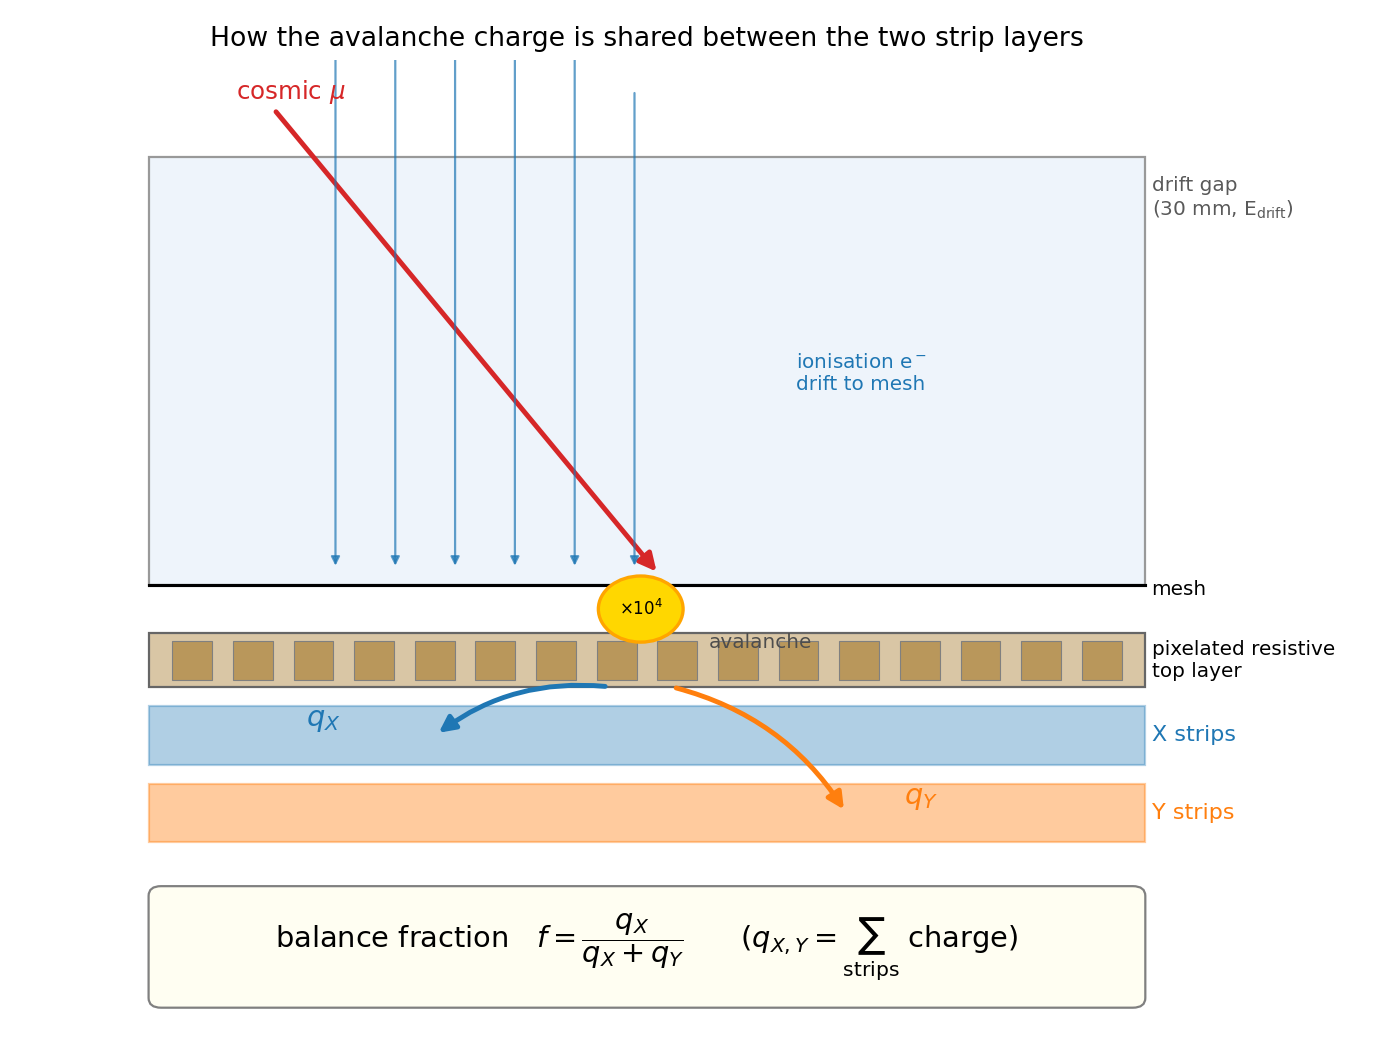
\includegraphics[width=0.82\textwidth]{schematic_routing.png}
  \caption{The physics. A cosmic muon ionises the drift gap; the electrons drift
  to the mesh and avalanche ($\times10^4$); the avalanche charge is collected on
  the pixelated resistive top layer, which routes it to the X strips and to the
  Y strips underneath. The balance fraction $\fbal=\qx/(\qx+\qy)$
  [Eq.~\eqref{eq:f}] measures how that single avalanche is divided between the
  two readout layers.}
  \label{fig:routing}
\end{figure}

\section{What we measure, and how}
\label{sec:metrics}

\paragraph{Charge per plane.} For each matched event we sum the reconstructed
charge over the fired strips of each plane (Eq.~\ref{eq:f}). Because the answer
should not depend on \emph{how} we weigh a strip's charge, we compute $\fbal$
three independent ways (Fig.~\ref{fig:metric}a): (i) the saturation-corrected
\textbf{peak amplitude} (the primary estimator; the reconstruction fits pulses
that clip the 12-bit ADC, so a saturated peak strip is still measured, not lost);
(ii) the \textbf{pulse integral} (area under the waveform = collected charge,
evaluated on unsaturated events where the area is unbiased); and (iii) the
\textbf{clustered unshared strip sum} \texttt{amp\_sum} from the micro-TPC
segment fit (spark-free, already de-shared). Agreement among the three shows
$\fbal$ is a property of the detector, not of the estimator.

\paragraph{The metrics.} From the per-event $(\qx,\qy)$ pairs we report
(Fig.~\ref{fig:metric}b,c):
\begin{itemize}\itemsep2pt
  \item the \textbf{correlation} of $\qx$ and $\qy$ (2-D distribution and
        Pearson $r$) --- both layers sample one avalanche, so they must track
        each other;
  \item the \textbf{distribution of $\fbal$}: its median (the balance point) and
        its $\sigma_{68}$ half-width (the event-by-event sharing fluctuation ---
        \emph{this width is the design metric});
  \item the log-ratio $\ln(\qx/\qy)$, a symmetric, better-behaved companion to
        $\fbal$;
  \item the \textbf{map of median $\fbal$} over the active area --- flat = the
        pixel coupling is position-independent; its bin-to-bin scatter is
        compared against the scatter \emph{expected} from finite per-bin
        statistics, so only excess counts as real non-uniformity;
  \item the dependence of $\fbal$ on \textbf{track angle} $|\tan\theta|$ and on
        \textbf{total charge} $\qx+\qy$ (a linearity/saturation check).
\end{itemize}

\begin{figure}[h]
  \centering
  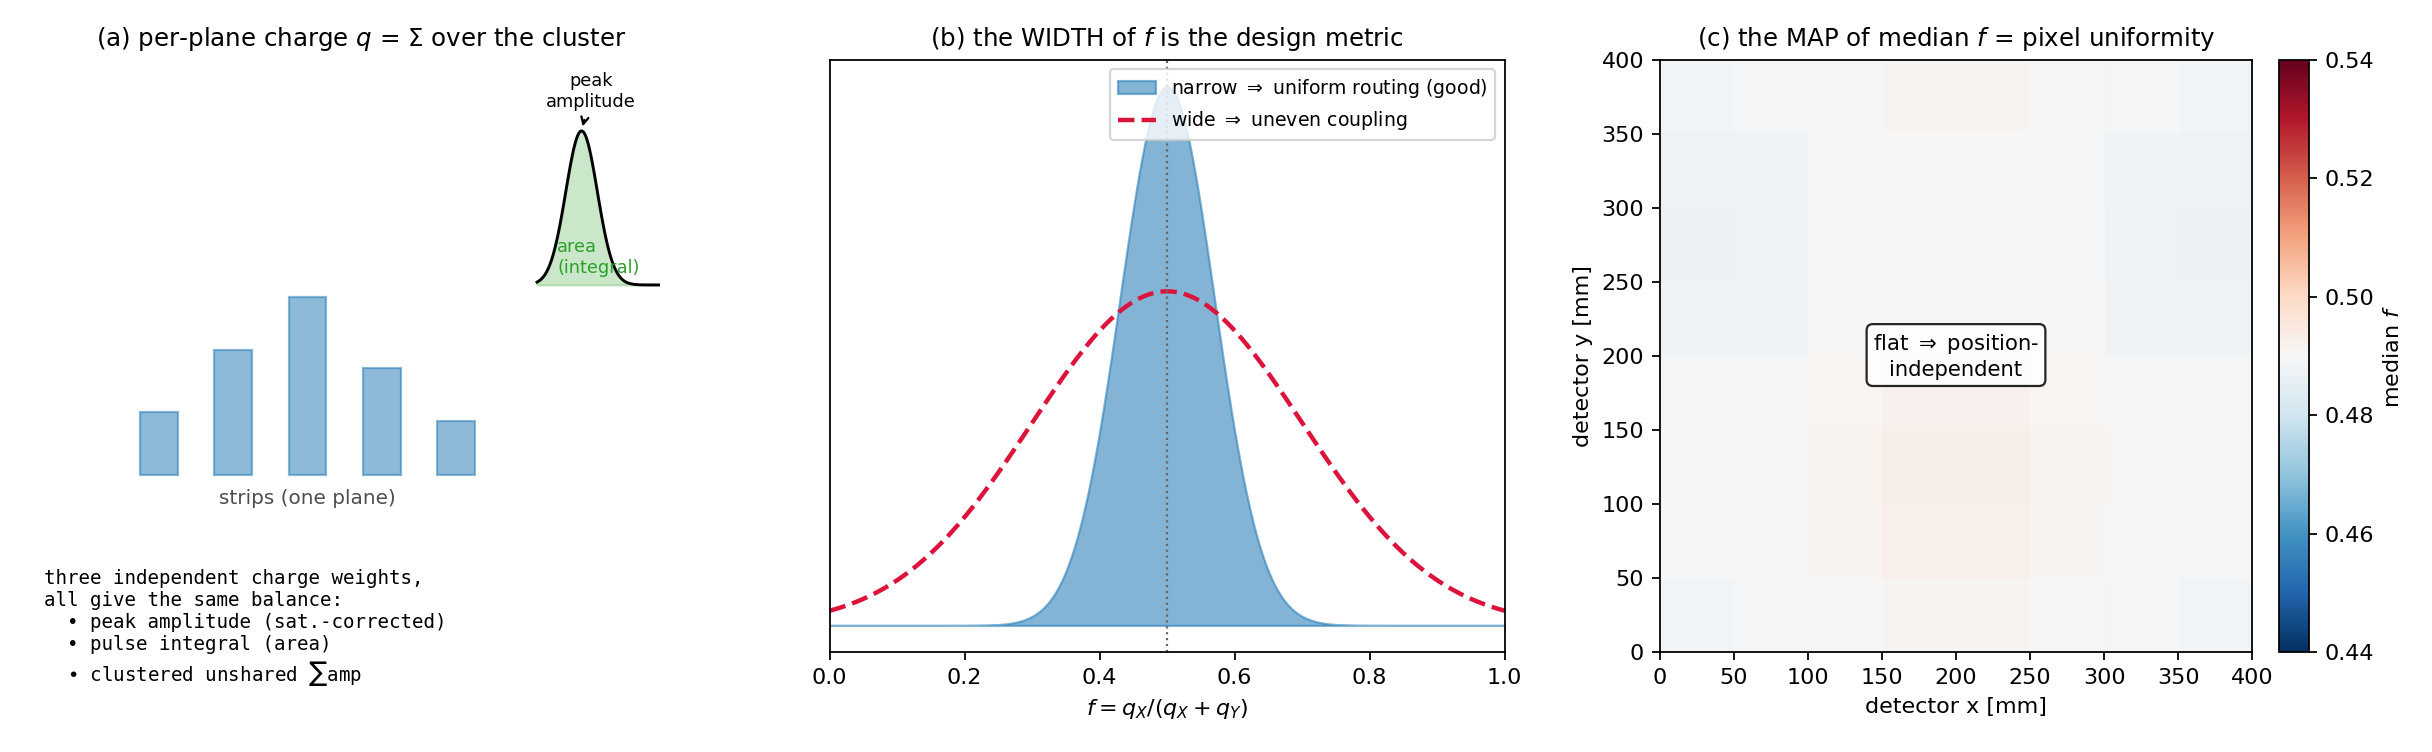
\includegraphics[width=\textwidth]{schematic_metric.png}
  \caption{What the metrics mean. \textbf{(a)} The per-plane charge is the sum
  over the strip cluster; each strip's charge is weighed three independent ways
  (peak amplitude, pulse area/integral, clustered de-shared sum). \textbf{(b)}
  The \emph{width} of the $\fbal$ distribution is the quantity of interest:
  narrow $\Rightarrow$ uniform routing (good); wide $\Rightarrow$ uneven pixel
  coupling. \textbf{(c)} The \emph{map} of median $\fbal$ tests position
  independence --- a flat map means the split does not depend on where the muon
  crossed.}
  \label{fig:metric}
\end{figure}

\paragraph{Data sample.} det3 is the Saturday scan run \texttt{sat\_det3}
(\texttt{mx17\_det3\_saturday\_scan\_6-27-26}, operating point resist
\SI{490}{V} / drift \SI{1000}{V}, FEU~7\,=\,X / 8\,=\,Y); det2 is the
overnight run \texttt{o22\_long\_det2} (resist \SI{525}{V}, FEU~6\,=\,X / 8\,=\,Y),
both Ar/iC$_4$H$_{10}$ 95/5. We select events with a single clean M3 telescope
ray (v2 recipe $\chi^2<1.0$, $N_\mathrm{clus}=4$; since 2026-07-14, was $\chi^2<5$,
$N_\mathrm{clus}\ge3$), both planes fired, a hit
within \SI{10}{mm} of the ray, and the hit inside the active area with a
\SI{5}{mm} fiducial margin (in the detector strip frame; the \SI{0}{}--\SI{25}{mm}
degrader fringe is discussed but not used for the core numbers). Spark events are
removed by the standard $>\!50$-strip multiplicity veto; only genuine
pulse-fit divergences (per-strip amplitude $>5\times10^4\adc$; 1--4 events per
run) are dropped. This yields $15\,129$ core events (det3) and $10\,589$ (det2).

\section{Results}

\subsection{The two layers see the same avalanche}
Figure~\ref{fig:corr} shows $\qx$ versus $\qy$ for det3. The charge lies along a
tight ridge with Pearson $r=0.881$ (det2: $0.846$): whenever one layer sees a
large signal, so does the other, as required if both sample one avalanche. The
ridge sits marginally \emph{above} the $\qx=\qy$ diagonal, i.e.\ $\fbal$ slightly
below $0.5$ --- Y collects a touch more charge on det3.

\begin{figure}[h]
  \centering
  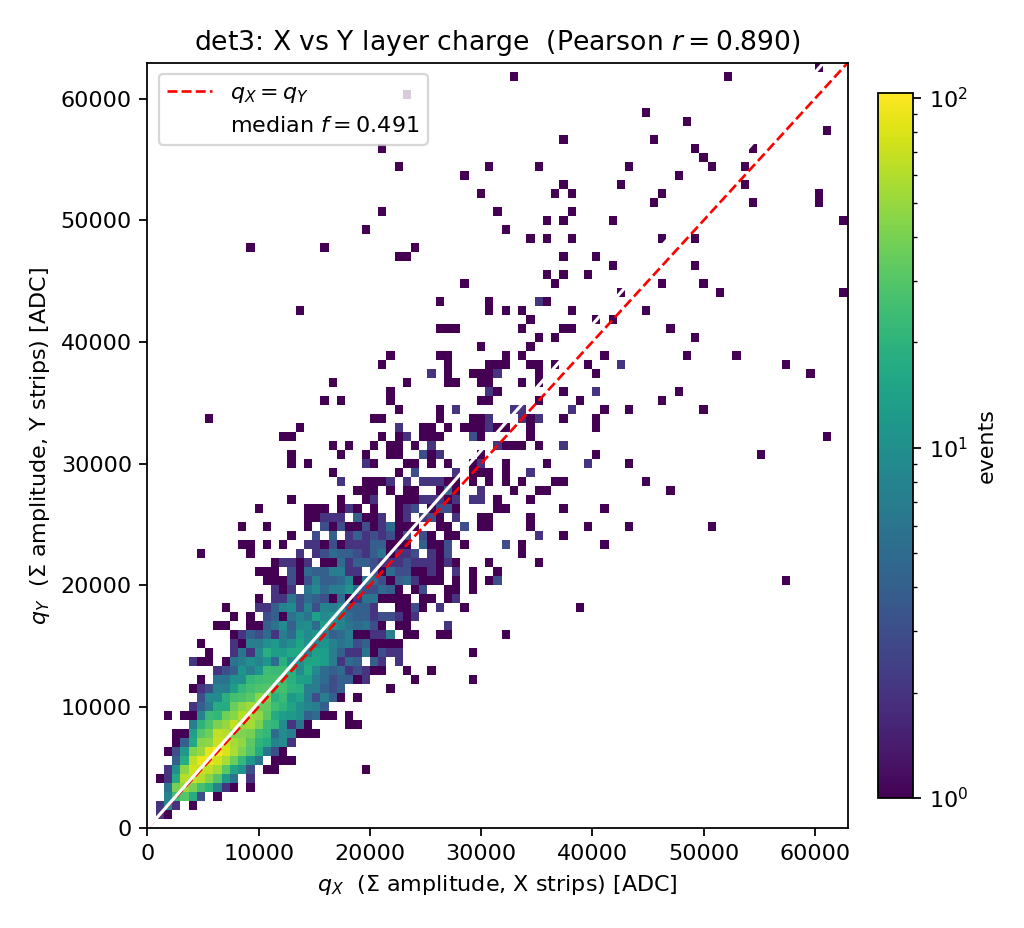
\includegraphics[width=0.6\textwidth]{qx_vs_qy.png}
  \caption{det3: per-event X-layer charge $\qx$ vs Y-layer charge $\qy$
  (saturation-corrected amplitude sums). The tight correlation ($r=0.881$)
  confirms both layers read one avalanche; the white line is the median-$\fbal$
  ray, just off the $\qx=\qy$ diagonal (dashed).}
  \label{fig:corr}
\end{figure}

\subsection{The balance is even and narrow}
The $\fbal$ distribution (Fig.~\ref{fig:dist}b) is narrow and centred near $0.5$:
median $0.487$, $\sigma_{68}=0.067$ (det3); $0.531$, $0.071$ (det2). The two
chambers are offset by only ${\sim}0.04$ --- det3 favours Y slightly, det2
favours X slightly --- while both widths are essentially identical. A
${\sim}4\%$ chamber-to-chamber offset with a $7\%$ intrinsic width is exactly the
signature of a well-coupled readout with a small per-assembly bias: the
\emph{constancy}, not the central value, carries the physics.

The three independent charge estimators agree on the balance point
(Fig.~\ref{fig:dist}a): for det3 the medians are $0.487$ (amplitude), $0.480$
(integral), $0.488$ (segment) --- a spread of $\le0.008$; for det2 they are
$0.531/0.527/0.509$. The integral distribution is intrinsically tighter
(area averages out peak noise), but its \emph{centre} matches, so the measured
balance is not an artefact of the peak-amplitude estimator. Table~\ref{tab:res}
collects the numbers.

\begin{figure}[h]
  \centering
  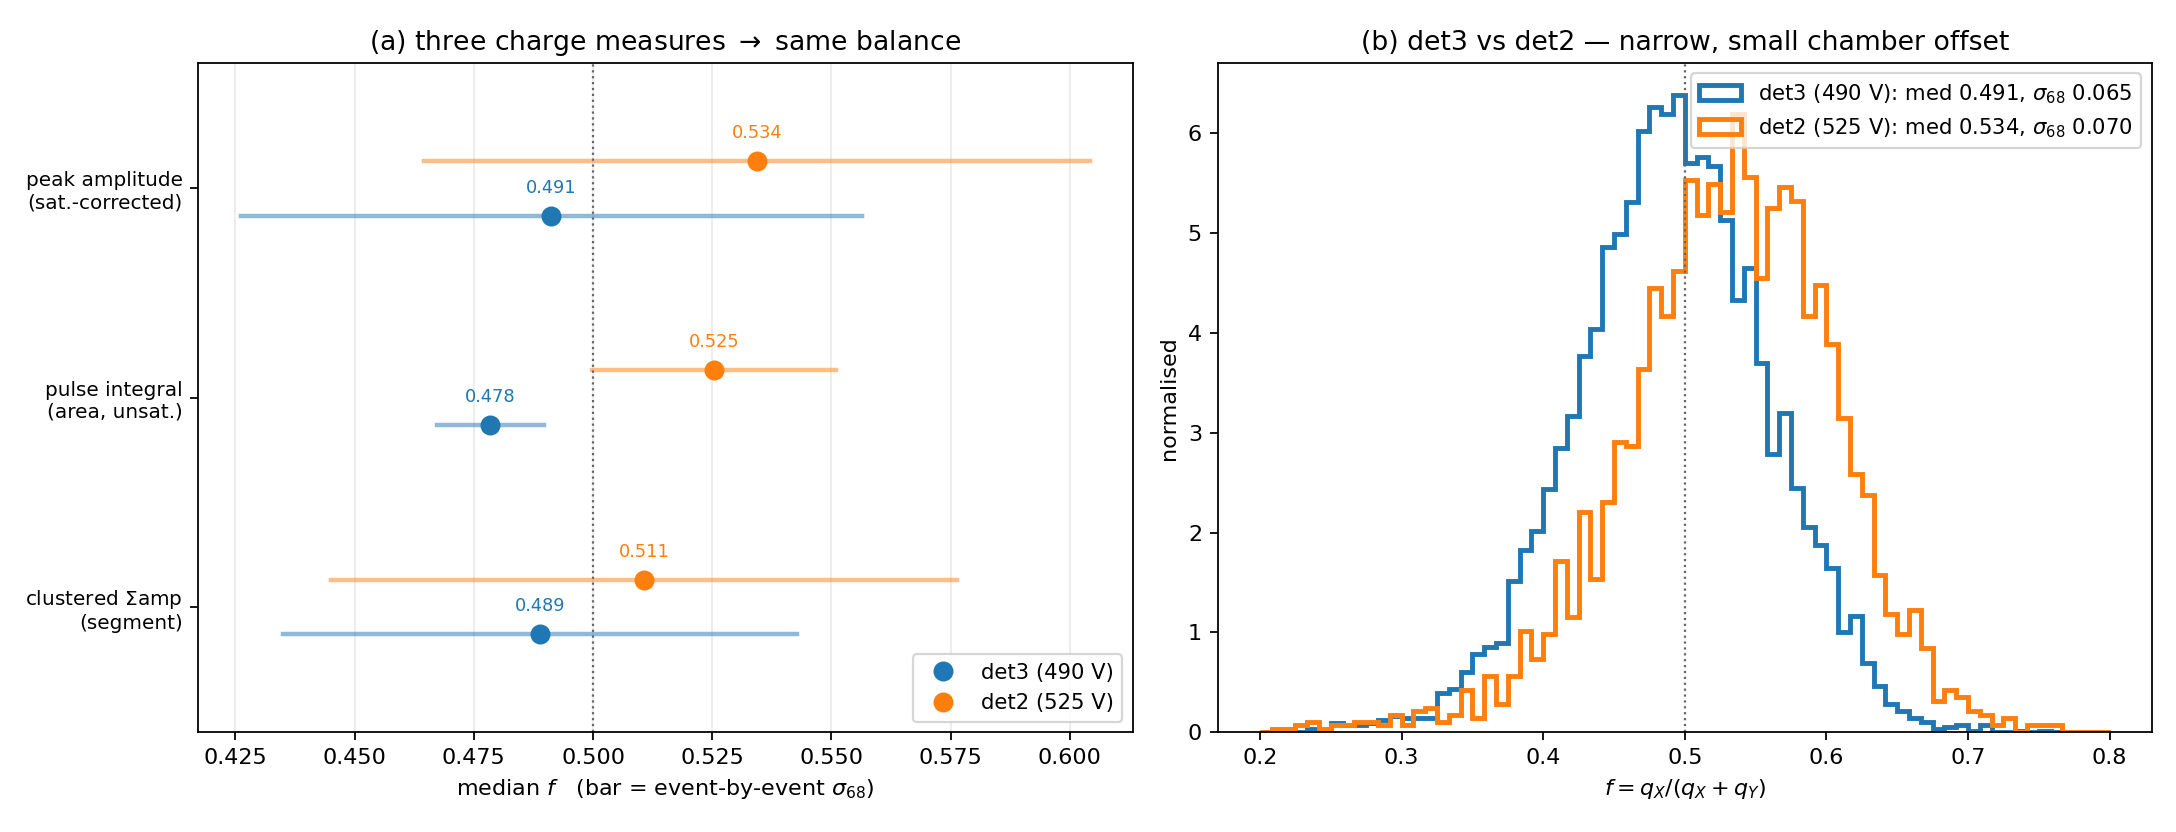
\includegraphics[width=\textwidth]{f_distribution.png}
  \caption{\textbf{(a)} The balance point is the same for all three charge
  estimators, per detector (markers = median $\fbal$; bars = event-by-event
  $\sigma_{68}$). det3 clusters just below $0.5$, det2 just above.
  \textbf{(b)} Full $\fbal$ distributions: narrow ($\sigma_{68}\approx0.07$),
  with the small det3/det2 offset visible as a shift, not a broadening.}
  \label{fig:dist}
\end{figure}

\begin{table}[h]
  \centering
  \caption{Charge-balance summary. $\fbal=\qx/(\qx+\qy)$; $\sigma_{68}$ is the
  distribution half-width. ``inner std'' is the bin-to-bin scatter of the
  median-$\fbal$ map over the fiducial core, with the value \emph{expected} from
  finite per-bin statistics in parentheses --- the real position variation is
  $\sqrt{\text{std}^2-\text{stat}^2}\approx0.018$ for both.}
  \label{tab:res}
  \sisetup{table-format=1.3}
  \begin{tabular}{lcc}
    \toprule
    quantity & det3 (\texttt{sat\_det3}, \SI{490}{V}) & det2 (\texttt{o22\_long\_det2}, \SI{525}{V})\\
    \midrule
    core events                     & $15\,129$ & $10\,589$ \\
    median $\fbal$ (amplitude)       & $0.487$ & $0.531$ \\
    $\sigma_{68}(\fbal)$             & $0.067$ & $0.071$ \\
    median $\fbal$ (integral)        & $0.480$ & $0.527$ \\
    median $\fbal$ (segment $\Sigma$amp) & $0.488$ & $0.509$ \\
    Pearson $r(\qx,\qy)$             & $0.881$ & $0.846$ \\
    $\ln(\qx/\qy)$ median            & $-0.052$ & $+0.122$ \\
    slope $\mathrm{d}\fbal/\mathrm{d}|\tan\theta|$ & $+0.021$ & $-0.003$ \\
    $\fbal$-map inner std (stat.)    & $0.020\ (0.009)$ & $0.021\ (0.011)$ \\
    saturation systematic $\Delta\fbal_{\text{sat}-\text{clean}}$ & $-0.007$ & $-0.037$ \\
    \bottomrule
  \end{tabular}
\end{table}

\subsection{The balance does not depend on position}
Figure~\ref{fig:maps} maps the median $\fbal$ across the active area of each
chamber. The core is flat: the bin-to-bin standard deviation over the fiducial
region is $0.020$ (det3) / $0.021$ (det2), against $0.009$ / $0.011$ expected
from the finite number of events per bin. The real position variation is
therefore only $\sqrt{0.020^2-0.009^2}\approx0.018$ --- about $2\%$ of the
central value, i.e.\ the pixel coupling is uniform to the few-percent level. The
visible structure sits at the top-$y$ / low-$x$ edges: this is the known
degrader-fringe and bad-strip band (the same $\lesssim\SI{25}{mm}$ edge that
drives the efficiency turn-on and angle distortion elsewhere in the analysis),
and it is excluded from the core statistic rather than averaged in.

\begin{figure}[h]
  \centering
  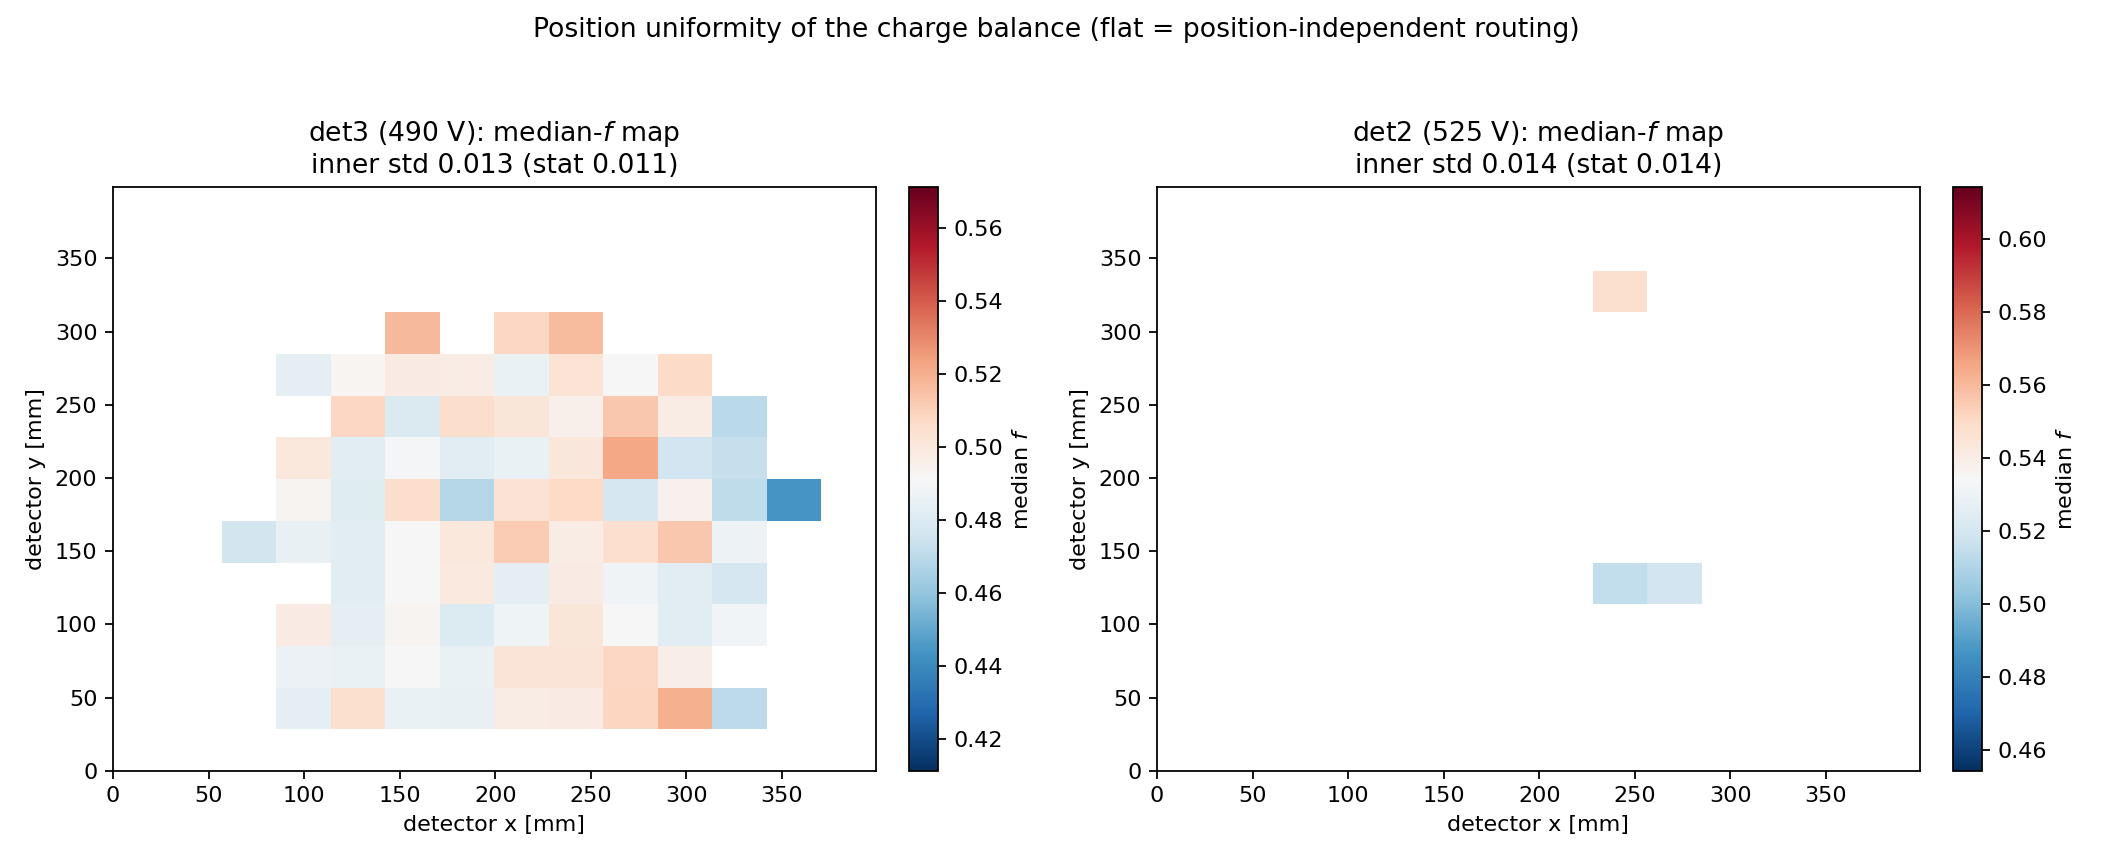
\includegraphics[width=\textwidth]{f_maps.png}
  \caption{Median-$\fbal$ map over the active area for det3 (left) and det2
  (right). The colour scale spans $\pm0.08$ about each chamber's central
  $\fbal$. The core is flat to ${\sim}2\%$ (inner std vs.\ statistical
  expectation quoted in each title); the coloured band at the top edge is the
  known degrader-fringe / bad-strip region, excluded from the core number.}
  \label{fig:maps}
\end{figure}

\subsection{Stable in angle and charge; saturation is benign}
Figure~\ref{fig:stab} closes the robustness checks.
\textbf{(a)} $\fbal$ is flat versus track inclination $|\tan\theta|$ (slope
$+0.021$ det3, $-0.003$ det2): inclined tracks spread charge over more strips and
pixels, yet the X/Y split is unchanged --- the routing is a property of the pixel
layer, not of the track topology.
\textbf{(b)} Splitting det3 by whether any strip saturated shows the two
populations track each other to within the quoted systematic
($\Delta\fbal_{\text{sat}-\text{clean}}=-0.007$ for det3; $-0.037$ for the
higher-gain det2, where the saturation correction works harder). Because the
amplitude is saturation-corrected, keeping these events (rather than discarding
the ${\sim}40\%$ of tracks whose peak strip clips) avoids a low-charge selection
bias, and the split confirms the correction does not distort $\fbal$.
\textbf{(c)} The width $\sigma_{68}(\fbal)$ shrinks with total charge, as
expected for a fluctuation dominated by per-strip noise, reaching ${\sim}0.057$
for the largest signals.

\begin{figure}[h]
  \centering
  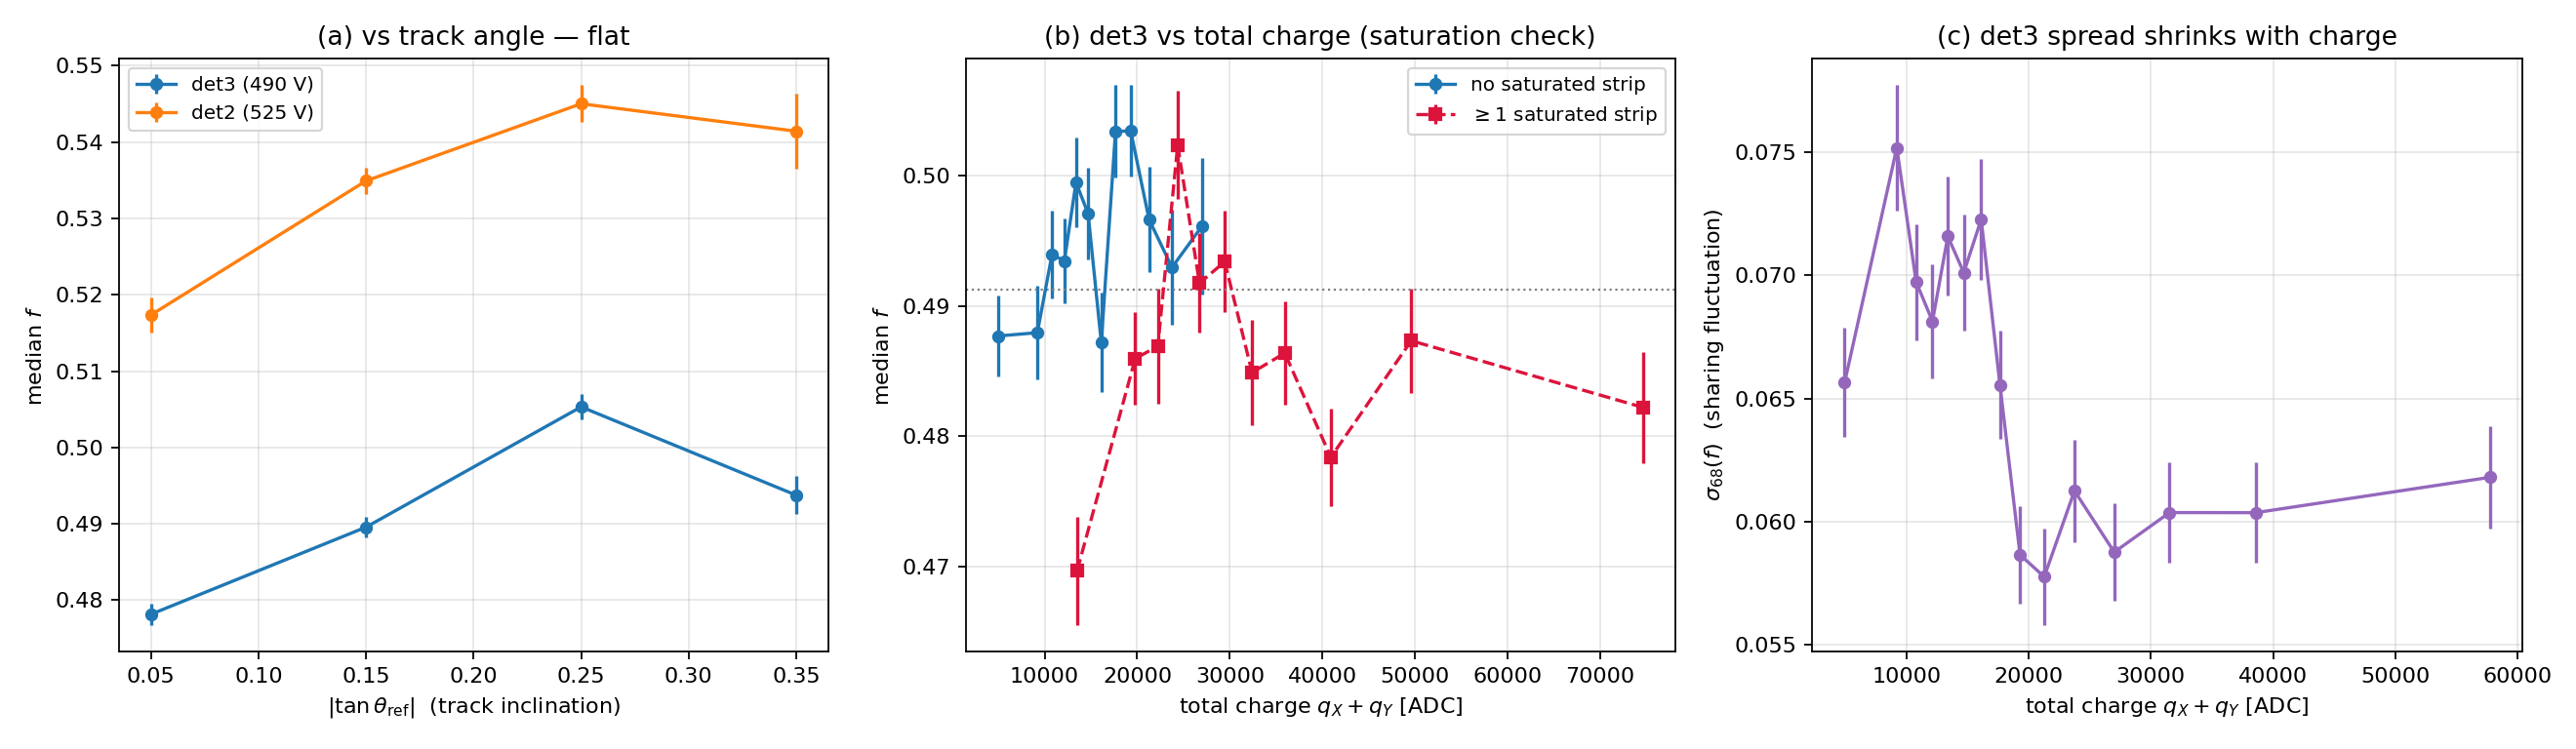
\includegraphics[width=\textwidth]{f_stability.png}
  \caption{\textbf{(a)} median $\fbal$ vs track angle --- flat for both chambers.
  \textbf{(b)} det3 $\fbal$ vs total charge, split by saturated-strip presence:
  the saturation correction leaves $\fbal$ unbiased to the quoted systematic.
  \textbf{(c)} the sharing fluctuation $\sigma_{68}(\fbal)$ decreases with signal
  size.}
  \label{fig:stab}
\end{figure}

\section{Conclusion}
The pixelated resistive top layer of the MX17 chamber divides each avalanche
\textbf{evenly and uniformly} between the X and Y strip layers. The balance
fraction $\fbal=\qx/(\qx+\qy)$ is narrow ($\sigma_{68}\approx0.07$), flat in
position (real variation $\approx2\%$) and in angle, and centred near $0.5$ with
only a small per-chamber offset ($0.487$ det3, $0.531$ det2). The conclusion is
robust: it holds for three independent charge estimators, survives the saturation
correction, and reproduces across two detectors at different gains. This is the
behaviour required for balanced two-coordinate readout, and it closes the last
previously-unmeasured item on the June micro-TPC paper list.

\vspace{0.5em}
\footnotesize\noindent\textit{Reproduce:} from \texttt{mx\_june\_cosmic\_qa/},
\texttt{../.venv/bin/python 38\_xy\_charge\_balance.py o22\_long\_det2} then
\texttt{sat\_det3} (streams \texttt{combined\_hits}, writes per-run
\texttt{charge\_balance/} outputs + the per-event cache), then
\texttt{38b\_charge\_balance\_report\_figs.py} for the figures in this report.

\end{document}
